\documentclass[10pt, letterpaper]{article}
\usepackage[utf8]{inputenc}
\usepackage{amsmath}
\usepackage{amssymb}
\usepackage{bbm}
\usepackage{booktabs}
\usepackage{caption}
\usepackage{color}
\usepackage[shortlabels]{enumitem}
\usepackage{fancyhdr}
\usepackage{hyperref}
\usepackage{geometry}
\geometry{a4paper,scale=0.8}
\usepackage{graphicx}
\graphicspath{ {./img/}}
\usepackage{listings}
\usepackage{mathtools}
\usepackage{mathrsfs}
\usepackage{setspace}
\renewcommand{\baselinestretch}{1.3}

% set-up header & footer
\pagestyle{empty}
\fancyhf{}
\cfoot{\thepage}
\lhead{%
\textbf{University of California, Berkeley} \\
Department of Civil \& Environ. Eng.
}
\rhead{\textbf{CS 285 Deep Reinforcement Learning}\\\date{\today}}

\title{%
    \textbf{Homework 3}
}
\author{Juanwu Lu (3037432593)\\ \small(M.Sc. Civil Engineering, UC Berkeley)}
\date{}

% set-up code listing
\definecolor{dkgreen}{rgb}{0,0.6,0}
\definecolor{gray}{rgb}{0.5,0.5,0.5}
\definecolor{manuve}{rgb}{0.58,0,0.82}

\lstset{frame=tb,
    language=Python,
    aboveskip=3mm,
    belowskip=3mm,
    showstringspaces=false,
    columns=flexible,
    basicstyle={\small\ttfamily},
    numbers=none,
    numberstyle=\tiny\color{gray},
    keywordstyle=\color{blue},
    commentstyle=\color{dkgreen},
    stringstyle=\color{manuve},
    breaklines=true,
    breakatwhitespace=true,
    tabsize=3
}

\begin{document}
\maketitle
\captionsetup[figure]{labelfont={bf},labelformat={default},labelsep=period,name={Figure}}
\captionsetup[table]{labelfont={bf},labelformat={default},labelsep=period,name={TABLE}}
\thispagestyle{fancy}
\pagestyle{plain}

% Part 1: Q-Learning
\section{Part 1: Q-Learning}

\subsection*{Question 1: basic Q-learning performance (DQN)}
\begin{figure}[thbp]
    \centering
    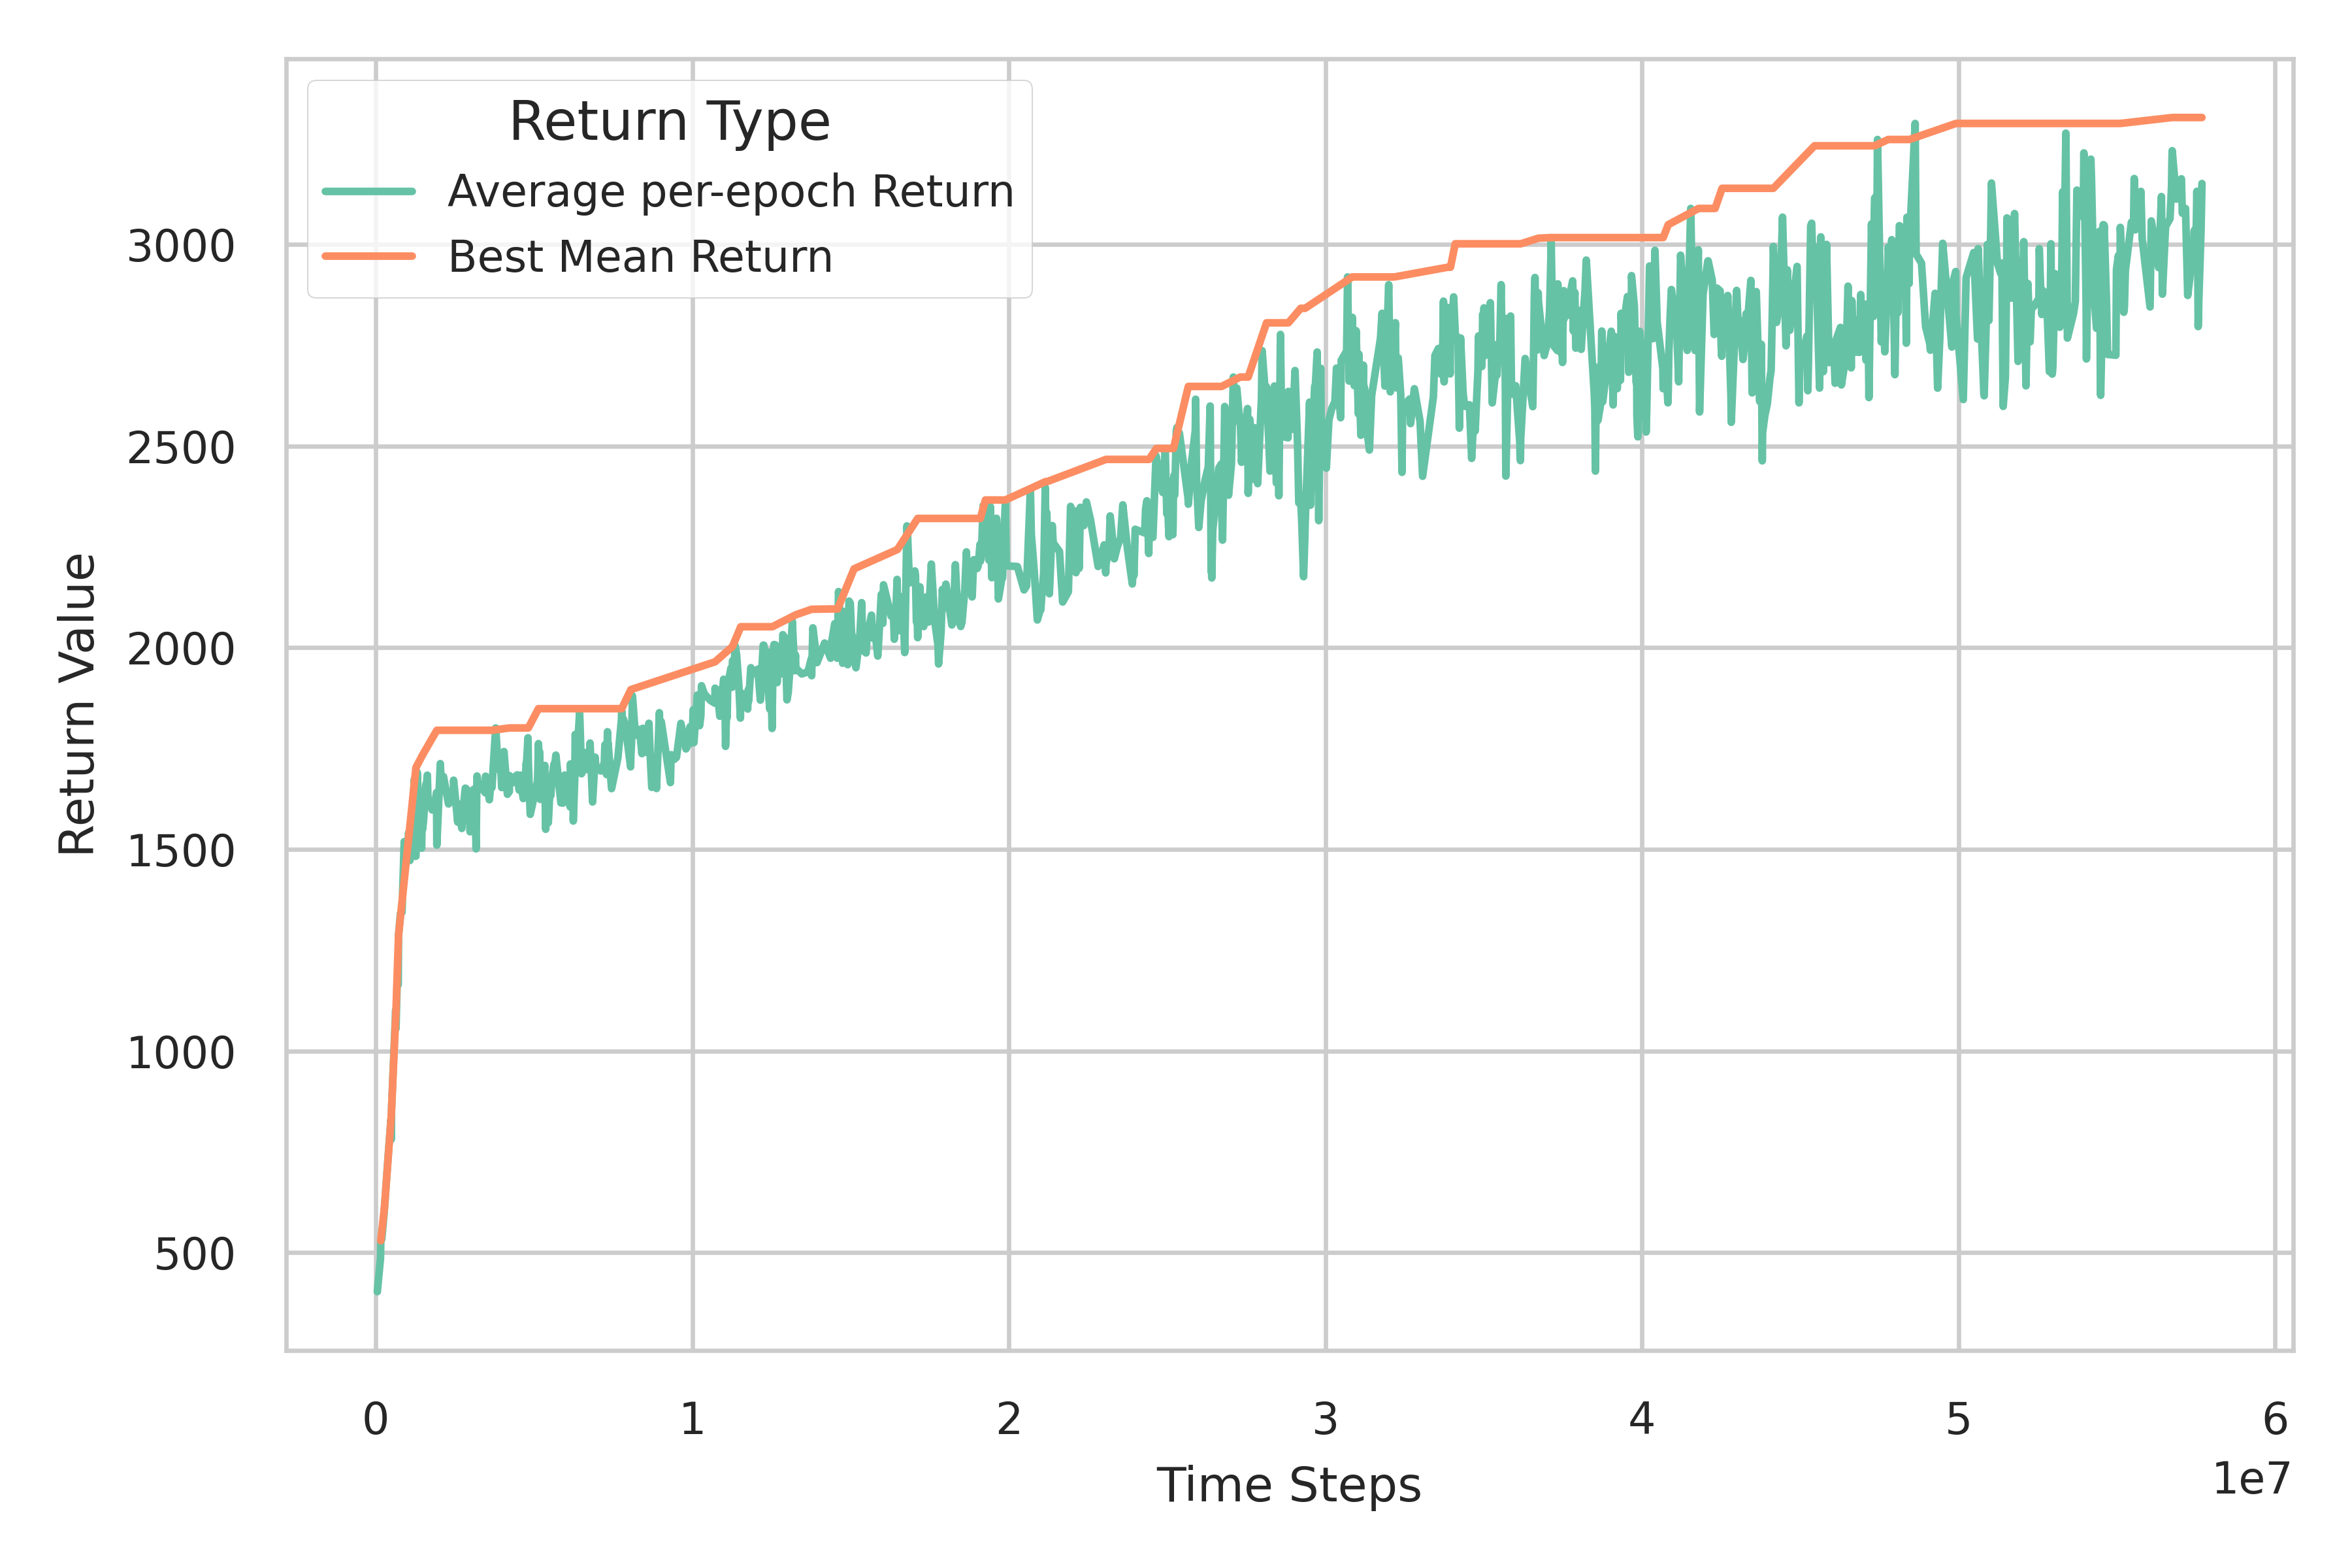
\includegraphics[width=\textwidth]{./img/q1.png}
    \caption{DQN performance on \texttt{Ms. Pac-Man} in average per-epoch return (cyan curve) and best mean return (red curve) versus number of time steps. Performance of the algorithm shows a step increasing trend. However, the average per-epoch return variances are also increasing.}
    \label{fig: 1}
\end{figure}

\pagebreak
\subsection*{Question 2: double Q-learning (DDQN)}
\begin{figure}[thbp]
    \centering 
    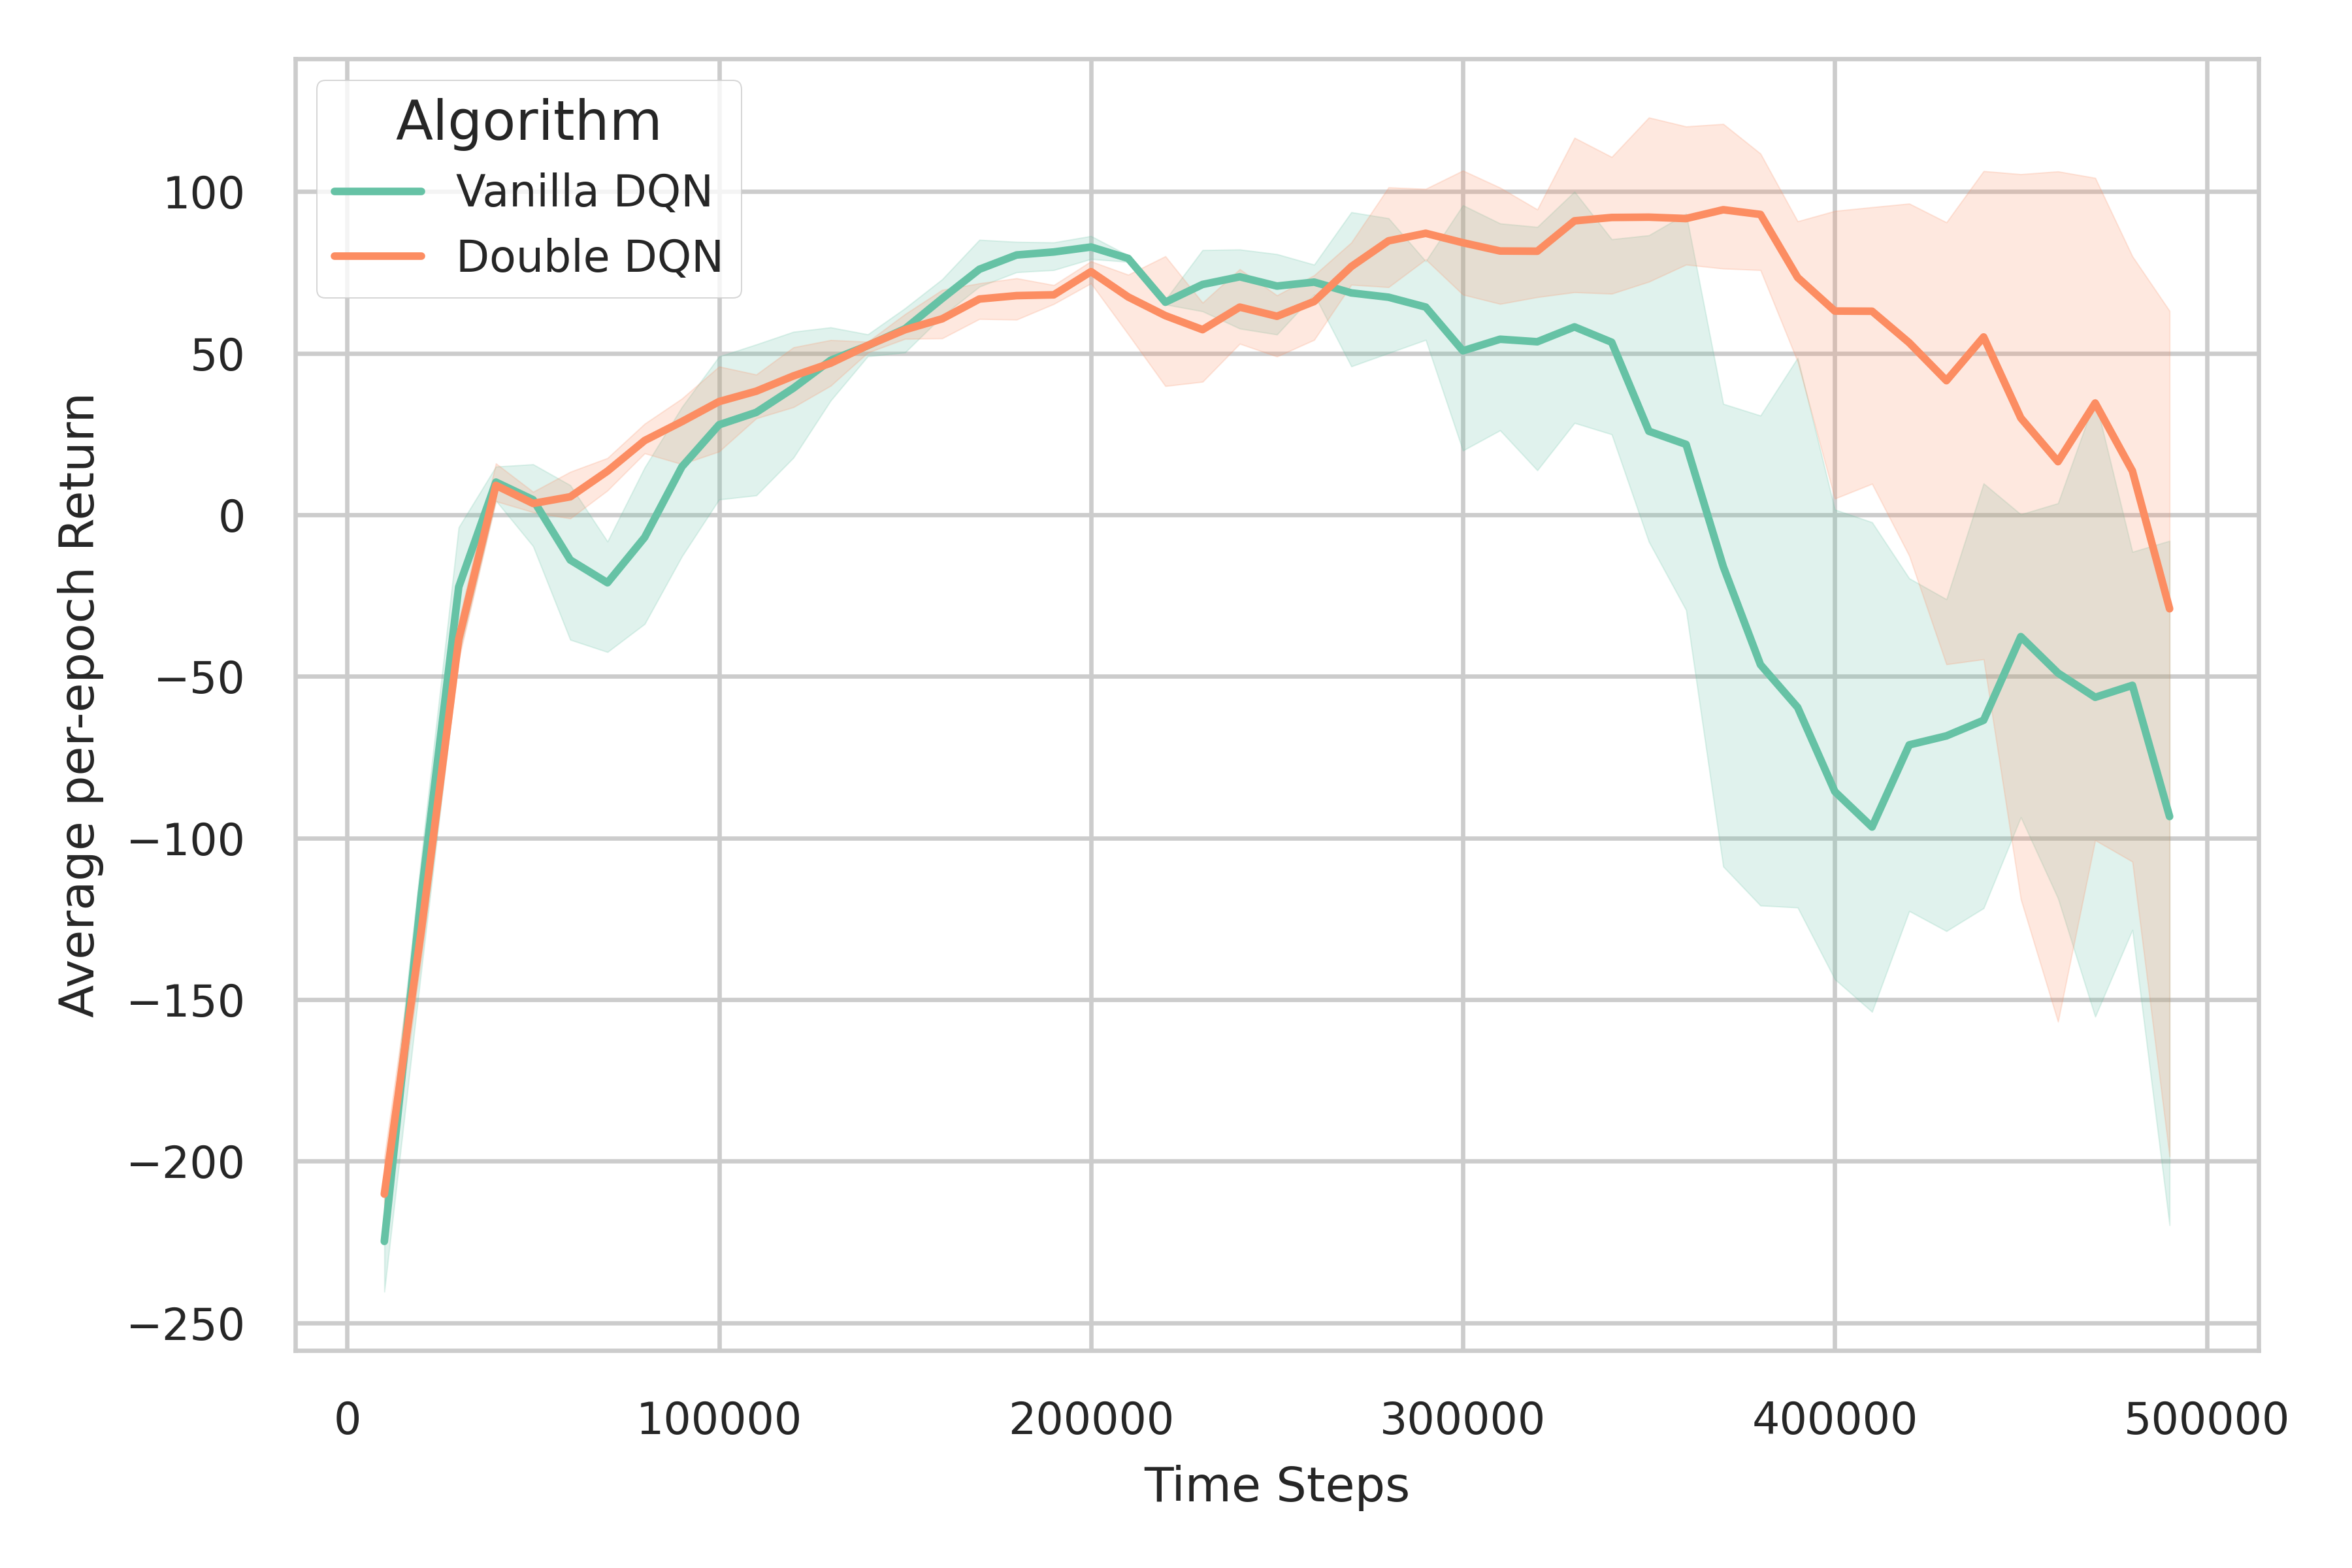
\includegraphics[width=\textwidth]{./img/q2.png}
    \caption{}
    \label{fig: 2}
\end{figure}

\subsection*{Question 3: experimenting with hyperparameters}
% figure

% Part 2: Actor-Critic
\newpage
\section{Part 2: Actor-Critic}

% Part 3: Soft Actor-Critic
\newpage
\section{Part 3: Soft Actor-Critic}

\end{document}